\documentclass[11pt, a4paper]{article}
\usepackage[utf8]{inputenc}
\usepackage[margin=1.2 in]{geometry}
\usepackage{graphicx}
\usepackage[T1]{fontenc}
\usepackage{charter}
\usepackage{amsmath}
\usepackage{setspace}
\usepackage{subcaption}
\usepackage{listings}
\graphicspath{{Assets/}}

\title{CSCU9YE Assignment Report}
\author{Student no: 2519302}
\date{November 17\textsuperscript{th} 2018}
\pagenumbering{roman}
\begin{document}
\begin{titlepage}
\maketitle
\clearpage\thispagestyle{empty}
\end{titlepage}
\doublespacing
\setstretch{2}
\tableofcontents
\thispagestyle{empty}
\newpage
\singlespacing

\section{Introduction}

This project is tasked with the classification of spam emails, to a high degree of accuracy using machine learning models. This report will aim to provide an overview of the datasets used, an understanding of how the models used work and the results obtained from running these models on the datasets mentioned.  
\section{Specification}

This section will walk through the flowchart shown in \emph{Figure~\ref{fig:flowchart}}.

\subsubsection*{Load Emails}

Firstly, the emails need to be loaded into the program in order to parse through them and begin the pre-processing stage. This involves reading in all the files in the folder and saving them to a variable for manipulation further on in the program. 

\subsubsection*{Pre-Process Data}

This stage is where the data is processed to convert case, remove elements such as punctuation and stop words and is where the process of lemmatization happens. This process is also referred to as normalization. These entities are removed due to their inherent lack of relevance to the end classification. Lemmatization on the other hand is done in order to reduce the complexity of the generated dictionary in the next step and thus  the overall runtime of the algorithms on the dataset.

\subsubsection*{Dictionary Creation}

This process, mentioned briefly above, entails the tallying of the most commonly occurring words in all the emails in the dataset. This is done such that a correlation can be obtained when reading through similar pieces of text. This allows us to see if the emails share similarities and thus may be classed under a label. The generated dictionary is then compared to the features extracted from each email.

\subsubsection*{Feature Extraction}

The feature extraction phase entails extracting a feature vector for all emails in the dataset. The features contain the number of occurrences of each entity in the email, with respect to the dictionary generated.  

\subsubsection*{Split Dataset}

The dataset is split into a test set and a training set. This is done such that the model can be trained on a subset of the dataset as a whole and the model can then be evaluated on the same data. The split is done at approximately 70 / 30, where the training set is 70\% of the full dataset and the remaining 30\% is used as the test set.

\subsubsection*{Train Model}

The models are trained with a subset of the dataset as mentioned above. 

\subsubsection*{Pre-Trained Model}

This process is where the pre-trained model is tested with the test set obtained from when the dataset was split.

\subsubsection*{Evaluate Trained Model}

The outputs of the models used here are evaluated using the performance matrices: Accuracy, Precision, Recall and F1-Score. The unlabelled dataset used here is the same test set, but without any accompanying labels designating the entities classification.

\subsection{Pseudocode}

\begin{lstlisting}[frame=single]
begin

    begin load_emails
        load emails into program
        split dataset into test set and training set
    end load_emails
	
    begin pre_processing
        convert text to lower case
        remove stop_words
        lemmatize text
    end pre_processing
	
    begin create_dictionary
        generate dictionary
    end create_dictionary
	
    begin feature_extraction
        extract feature vectors for all emails
    end feature_extraction
	
    Train models on training set
    Test models on test set
    Generate predictions using models
    Evaluate model predictions
    
end
\end{lstlisting}
\newpage
\begin{figure}[h!]
\centering
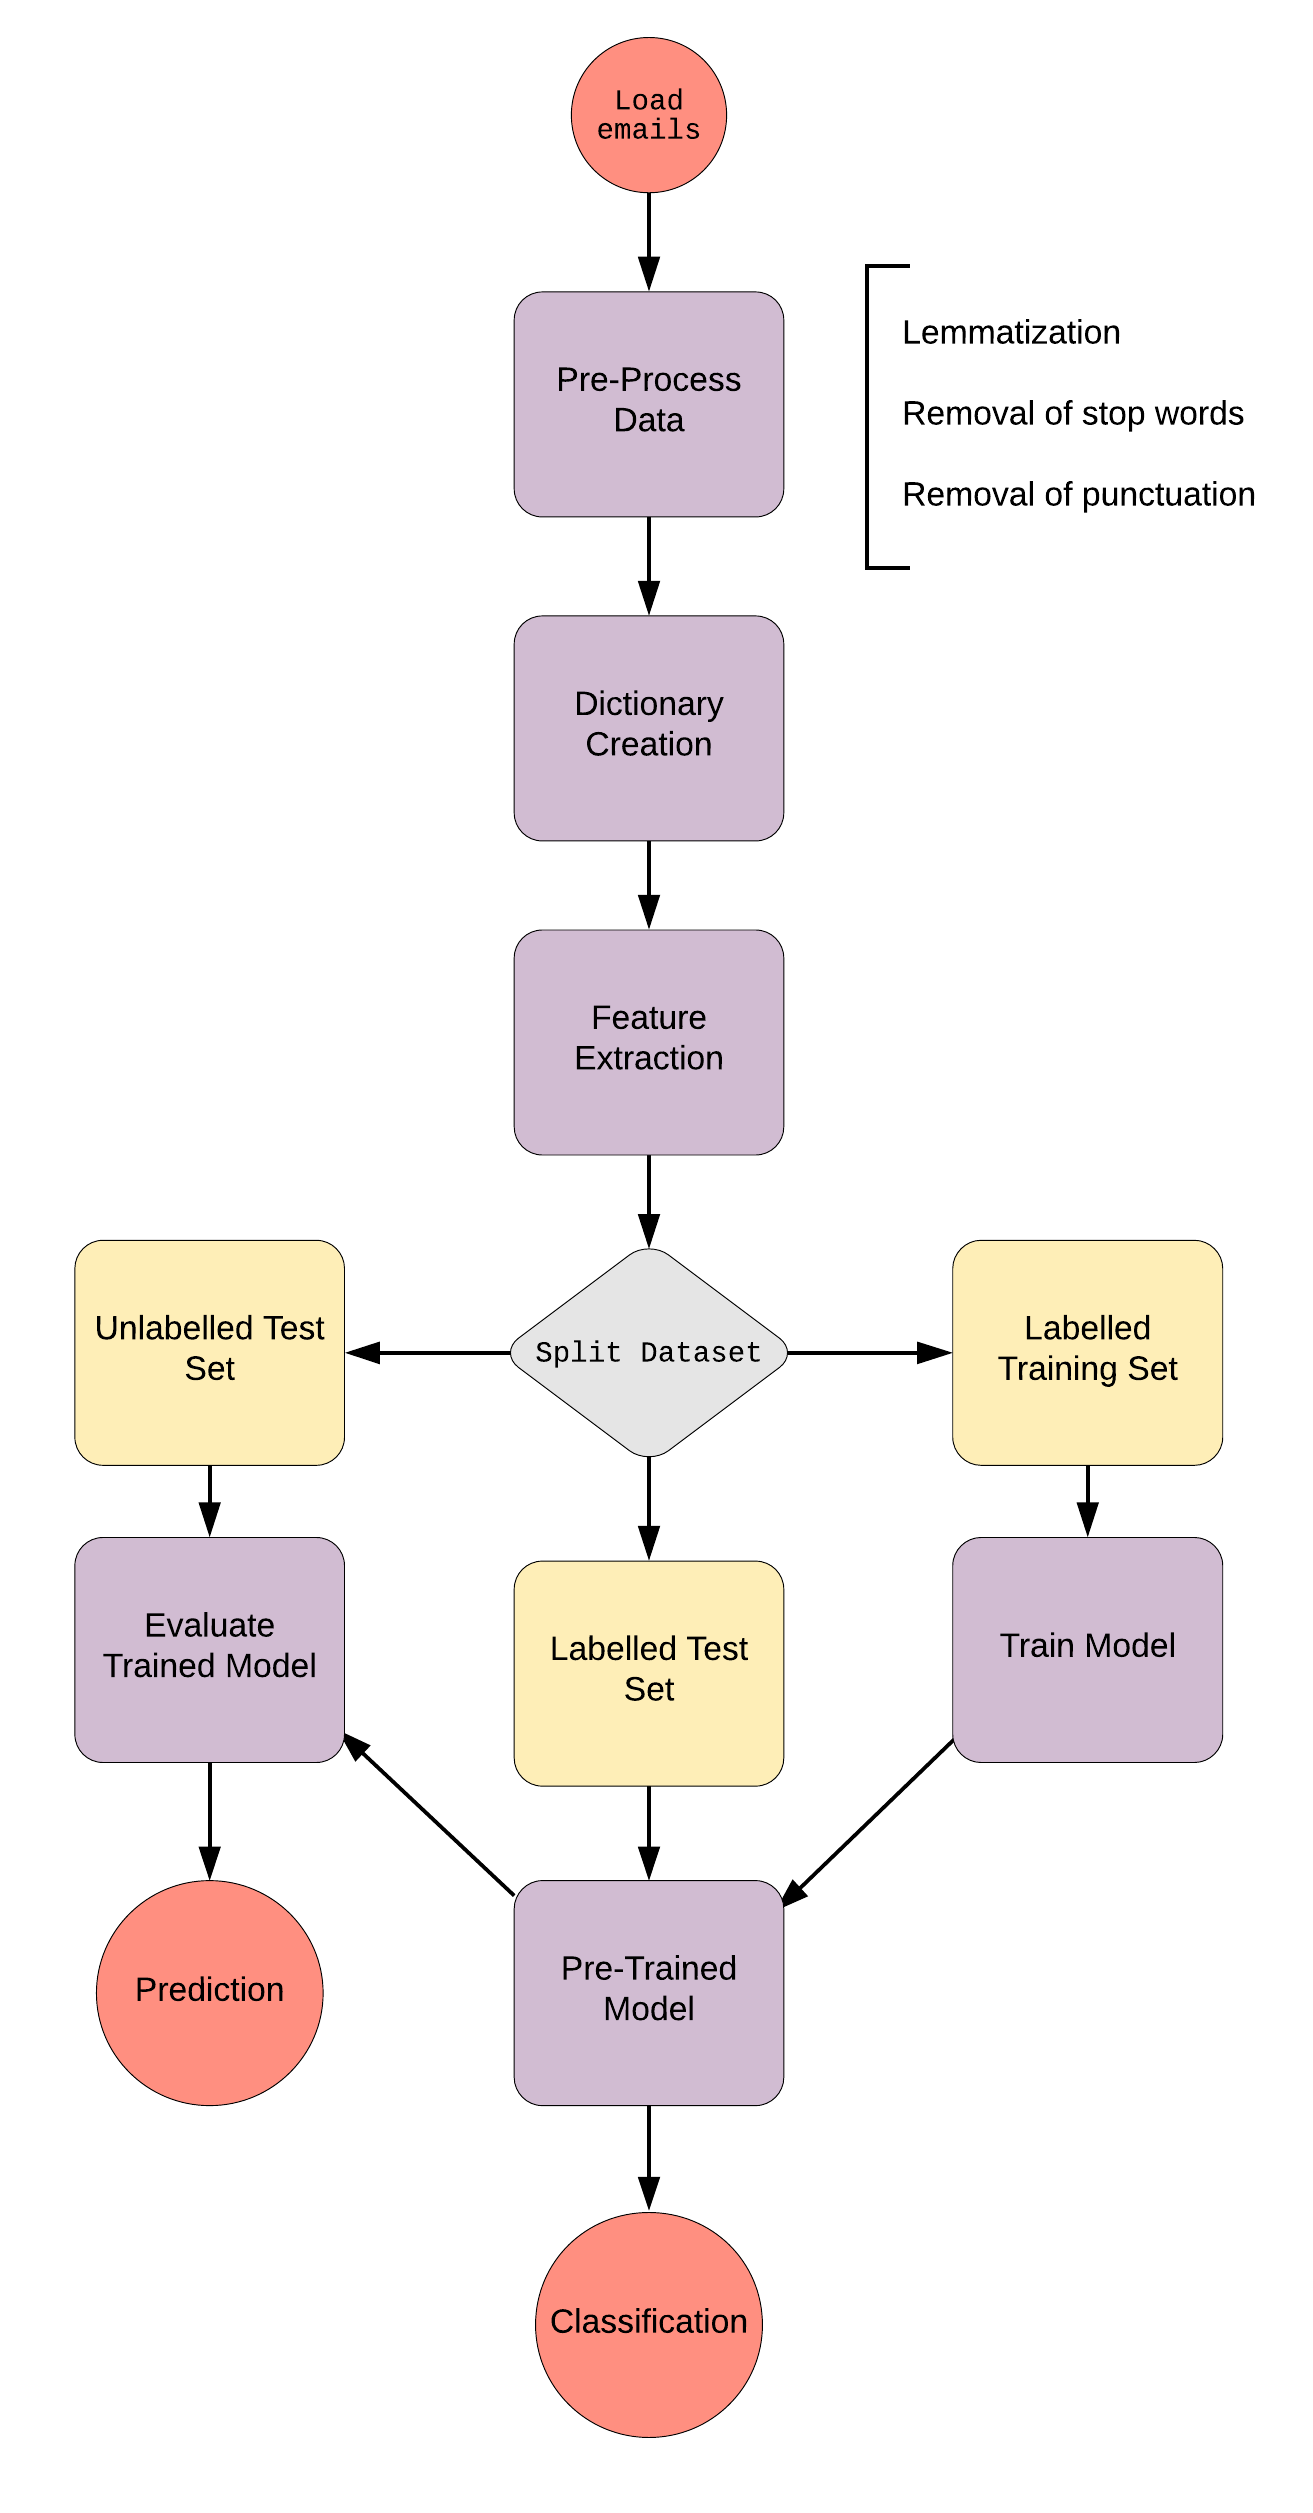
\includegraphics[scale=0.2]{spam_flowchart}
\caption{Flowchart for the general Spam Classification process}
\label{fig:flowchart}
\end{figure}
\newpage

\section{Pre-Processing}

This section will aim to cover the different aspects of pre-processing employed in this project. Within the datasets used in this project, we can see that the general steps one would need to take are as follows:
\begin{itemize}
\item Lemmatization
\item Removal of stop words
\item Removal punctuation
\end{itemize} 
Along with the aforementioned steps, the text will be processed to handle case. This is done by converting the text to lower case before any text normalization is done. 

\subsection{Lemmatization}

Lemmatization is a form of text normalization where the aim is to remove inflection and/or derive the base word from a family of words in the dataset \cite{schutze2008introduction,jabeen2018stem,fortney2017nlp}. The base of a word, is also known as the \textbf{lemma} or the \textbf{dictionary form}. This process also leads to a decrease in complexity during the runtime of the algorithm. An example of which is shown in \emph{Table \ref{table: lemma}} below.\\\\
Such mapping also allows us to find all relevant documents using a specific word.
\begin{table}[h!]
\centering
\begin{tabular}{c c c}
\hline
\textbf{Word} & & \textbf{Lemma}\\
\hline
\text{Cleaning} & \(\rightarrow\) & \text{Clean}\\
\hline
\text{Cleaner}  & \(\rightarrow\) & \text{Clean}\\
\hline
\text{Cleanliness} & \(\rightarrow\) & \text{Clean}\\
\hline
\end{tabular}
\caption{Showing the mapping of words to its lemma}
\label{table: lemma}
\end{table}

\subsection{Removal of Stop Words}

Stop words are words such as "the", "he" or "in". These words do not contribute to the overall meaning of the text and are thus removed during the pre-processing stage. This also tends to be done in order to improve indexing times for larger datasets.

\subsection{Removal of Punctuation}

Punctuation, like stop words are removed due to their lack of contribution to the overall understanding of the text.  

\section{Machine Learning Methods}

This section will aim to provide some knowledge on the machine learning models employed in this project. 

\subsection{Support Vector Machine}

A Support Vector Machine (SVM) is a discriminative classification method. This method produces a classification by finding an optimal hyperplane that segregates the data points and thus returns classifications \cite{svm}. This can be visualized easiest on a 2-Dimensional plot as can be seen below in \emph{Figure \ref{fig:svm}}:
\begin{figure}[h!]
\centering
\begin{minipage}[]{0.45\textwidth}
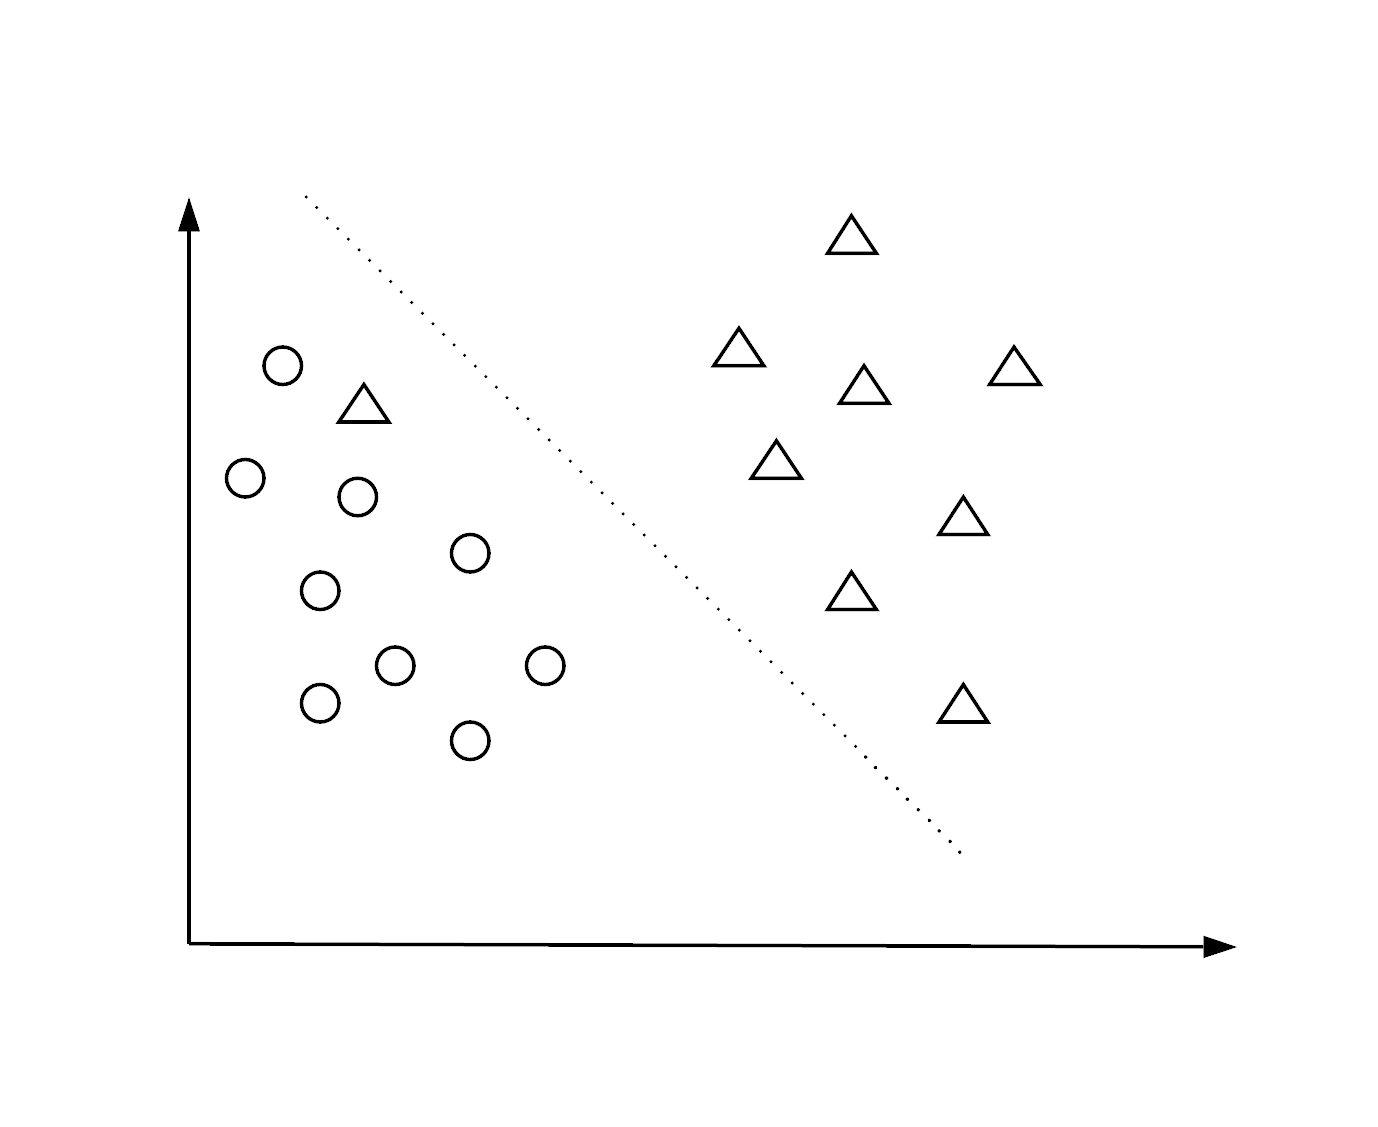
\includegraphics[scale=0.16]{svm}
\caption{SVM on 2-D plot area}
\label{fig:svm}
\end{minipage}
\hspace{0.5 cm}
\begin{minipage}[]{0.45\textwidth}
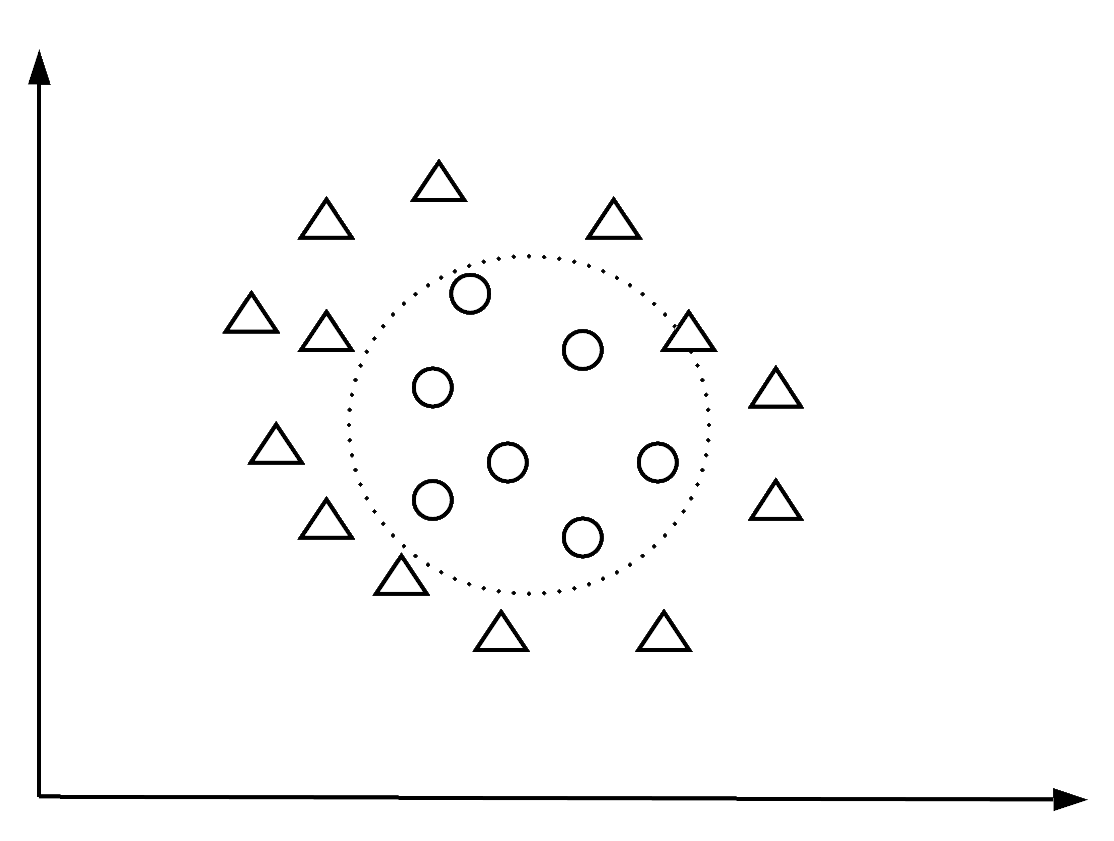
\includegraphics[scale=0.16]{svm_kernel}
\caption{Kernel feature of SVM}
\label{fig:svm_kernel}
\end{minipage}
\end{figure}

\emph{Figure \ref{fig:svm_kernel}} above shows an SVM making a classification on data where it would seem like there is no \emph{linear} hyperplane to be found. In order to make a classification, the SVM employs the kernel method \cite{ray2017svm}. This transformation, introduces a new dimension, by way of suggesting that for every \textbf{x} and \textbf{x'}, there is a function \emph{k} such that \emph{k} is equivalent to the sum of the squares of \textbf{x} and \textbf{x'} \cite{hofmann2008kernel}. This transformation then allows the model to find an optimal hyperplane within this third dimension. Transforming this back into a 2-Dimensional plot, the hyperplane is mapped as a circular boundary around the classified data points.

\subsection{Random Forest}

Random Forest is a supervised learning algorithm. The way it works is by generating a number of decision trees, all of which generate a classification. This is analogous to each decision tree in the forest 'voting' on a classification. The algorithm obtains a final singular classification by choosing the classification with the most 'votes'. To note, the decision trees generated by this algorithm are not pruned. 

\subsection{Multilayer Perceptron}

A Multilayer Perceptron (MLP), is a form of feedforward artificial neural network. 
  
%\section{Datasets Used} 

%\section{Measurement Metrics}

%\section{Results}
\newpage
\bibliography{references}
\bibliographystyle{ieeetr}
\end{document}
